\documentclass[12pt,a4paper]{article}

\usepackage[utf8]{inputenc}
\usepackage[T1]{fontenc}
\usepackage{mathpazo}
\usepackage[margin=1.15in]{geometry}
\usepackage{setspace}
\usepackage{hyperref}
\usepackage{titlesec}
\usepackage{amsmath,amsthm,amssymb}
\usepackage{booktabs}
\usepackage{enumitem}
\usepackage{fancyhdr}
\usepackage{xcolor}
\usepackage{tcolorbox}
\usepackage{tikz}
\usepackage{array}
\usepackage{float}

\newtcolorbox{vizpanel}[1][]{
  colback=gray!4, colframe=gray!50!black,
  fonttitle=\bfseries, title={Visualization: #1},
  sharp corners, boxrule=0.5pt
}

\hypersetup{colorlinks=true, linkcolor=blue!70!black, citecolor=black, urlcolor=blue!70!black}

\titleformat{\section}{\large\bfseries}{\thesection}{0.7em}{}
\titleformat{\subsection}{\normalsize\bfseries}{\thesubsection}{0.7em}{}
\titleformat{\subsubsection}{\normalsize\itshape}{\thesubsubsection}{0.7em}{}

\newtheorem{definition}{Definition}[section]
\newtheorem{proposition}[definition]{Proposition}
\newtheorem{theorem}[definition]{Theorem}
\newtheorem{lemma}[definition]{Lemma}
\newtheorem{corollary}[definition]{Corollary}
\newtheorem{example}[definition]{Example}
\theoremstyle{remark}
\newtheorem{remark}[definition]{Remark}

\newcommand{\R}{\mathbb{R}}
\newcommand{\ones}{\mathbf{1}}
\newcommand{\x}{\mathbf{x}}
\newcommand{\y}{\mathbf{y}}
\DeclareMathOperator*{\argmax}{arg\,max}

\newtcolorbox{intuition}[1][]{
  colback=blue!3, colframe=blue!40!black,
  fonttitle=\bfseries, title={Intuition: #1},
  sharp corners, boxrule=0.5pt
}
\newtcolorbox{keyinsight}[1][]{
  colback=orange!5, colframe=orange!60!black,
  fonttitle=\bfseries, title={Key Structural Insight},
  sharp corners, boxrule=0.5pt
}
\newtcolorbox{prebisch}[1][]{
  colback=green!3, colframe=green!40!black,
  fonttitle=\bfseries, title={Prebisch Connection: #1},
  sharp corners, boxrule=0.5pt
}

\setlength{\parindent}{1.5em}
\onehalfspacing
\setlength{\headheight}{14pt}
\pagestyle{fancy}
\fancyhf{}
\fancyhead[L]{\small\itshape Chapter 5: The Three Networks}
\fancyhead[R]{\small\thepage}
\renewcommand{\headrulewidth}{0.4pt}

\title{\vspace{-1cm}\textbf{Chapter 5} \\[0.5em]
\LARGE The Three Networks \\[0.3em]
\large\textit{Where the Structure Enters the Model}}
\author{}
\date{}

\begin{document}
\maketitle
\thispagestyle{fancy}

\begin{quote}
\textit{``Por dependencia entendemos una situaci\'{o}n en la cual la econom\'{i}a de ciertos pa\'{i}ses est\'{a} condicionada por el desarrollo y la expansi\'{o}n de otra econom\'{i}a a la cual la primera est\'{a} sometida.''}\\[0.3em]
\textnormal{[``By dependence we mean a situation in which the economy of certain countries is conditioned by the development and expansion of another economy to which the former is subjected.'']}\\
\hfill --- Theot\^{o}nio dos Santos, \textit{La estructura de la dependencia} (1970)
\end{quote}

\vspace{0.3em}

\begin{quote}
\textit{``Tell me who you walk with, and I'll tell you who you are.''}\\
\hfill --- Proverb, every language that has one
\end{quote}

\vspace{0.5em}

\begin{quote}
\textit{``Dime con qui\'{e}n andas y te dir\'{e} tu vector de Perron.''}\\
\hfill --- This book
\end{quote}

\vspace{1em}

Part~I showed that the standard competitive model assumes a specific interaction matrix --- $W = \frac{1}{N}\ones\ones'$ --- and that this assumption is what makes the welfare theorems hold. Part~II replaces that matrix with the one the world actually has.

This chapter introduces the three weight matrices that organize economic life:

\begin{enumerate}
\item $W^U$: the \textbf{utility network}. Who affects your wellbeing directly?
\item $W^P$: the \textbf{production network}. Who depends on whom for inputs and outputs?
\item $W^I$: the \textbf{information network}. Whose signals shape your beliefs and desires?
\end{enumerate}

Every economic interaction passes through at least one of these networks. Many pass through all three simultaneously. The salte\~{n}a vendor in La Paz is embedded in a production network (she buys flour from the miller, sells to the office worker), a utility network (her comadre's success makes her happy, her competitor's success makes her anxious), and an information network (she watches what other vendors charge, listens to the radio about the dollar exchange rate, hears from her cousin that there is work in El Alto). Her economic behavior --- what she produces, how she prices, whether she invests, what she wants for her daughter --- is determined not by her individual utility function in isolation but by her position in all three networks simultaneously.

The standard model collapses all three to $\frac{1}{N}\ones\ones'$ or ignores them entirely. This chapter makes them visible, distinct, and formal.

%% =====================================================================
\section{Before the Math: Three Stories}
\label{sec:stories}
%% =====================================================================

\subsection{The Utility Network: Keeping Up and Falling Behind}

Mar\'{i}a sells api on Calle Comercio. Her stall is between Doña Rosa's stall (empanadas) and Don Carlos's stall (newspapers). Mar\'{i}a has known Rosa for twenty years. They share a comadrazgo bond: Rosa is godmother to Mar\'{i}a's youngest daughter. When Rosa's sales are good, Mar\'{i}a feels genuinely happy for her. When Rosa's sales collapse --- say, because a new empanada chain opens nearby --- Mar\'{i}a worries, helps Rosa with a small loan, and feels the loss almost as her own.

Don Carlos, on the other hand, is just a neighbor. Mar\'{i}a doesn't dislike him, but his success or failure does not move her emotionally.

Now: how much of Rosa's consumption enters Mar\'{i}a's utility function? Quite a lot. How much of Carlos's? Almost nothing. How much of a stranger's in Santa Cruz? Zero.

This is the utility network $W^U$. Entry $W^U_{ij}$ measures how much agent $j$'s consumption or wellbeing directly affects agent $i$'s utility. For Mar\'{i}a: $W^U_{\text{Mar\'{i}a, Rosa}} \approx 0.3$ (strong positive externality), $W^U_{\text{Mar\'{i}a, Carlos}} \approx 0.02$ (negligible), $W^U_{\text{Mar\'{i}a, stranger}} = 0$.

In the standard model, $W^U = I$: your utility depends only on your own consumption. No externalities, no altruism, no envy, no keeping-up-with-the-Joneses. The salte\~{n}a vendor is an island.

\subsection{The Production Network: The Chain from Gas Well to Quinoa Bowl}

The gas well in Tarija produces natural gas. The gas goes to the processing plant (run by YPFB), which separates it into components. One component goes to the thermoelectric plant in Santa Cruz, which generates electricity. The electricity powers the flour mill in Cochabamba. The flour goes to the bakery. The bakery sells bread to the miner in Potos\'{i}. The miner extracts tin. The tin is exported. The export revenue enters the treasury. The treasury funds the school where Mar\'{i}a's daughter studies.

Each link in this chain is an entry in $W^P$. The gas well's output is an input to the processing plant: $W^P_{\text{plant, well}} > 0$. The processing plant's output is an input to the thermoelectric plant: $W^P_{\text{electric, plant}} > 0$. And so on. The chain from gas to quinoa bowl passes through six intermediate steps.

Now: how many of these links actually exist in Bolivia? The gas processing plant imports most of its equipment from Brazil. The thermoelectric plant was built by a Spanish firm. The flour mill buys Argentine wheat because Bolivian wheat production collapsed in the 1990s. At each step, the domestic chain breaks, and the production link points outward --- to the global economy rather than inward to the domestic economy.

This is Pinto's structural heterogeneity as a property of $W^P$: the off-diagonal entries between the gas block and the traditional block are tiny. The chain from gas well to quinoa bowl is mostly imaginary.

\subsection{The Information Network: What the Girl in Potos\'{i} Sees}

Mar\'{i}a's daughter, Luisa, is fifteen. She lives in Potos\'{i} and has a phone. On her phone she sees: TikTok videos from La Paz showing university students, Instagram posts from her cousin in Buenos Aires who is studying engineering, WhatsApp messages from her school friends who are all planning to finish secondary school and then --- what? Work in the market like their mothers? Go to the normal school in Sucre? Try for the public university in Oruro?

Twenty years ago, Luisa would have seen only what Potos\'{i} showed her: market vendors, miners, teachers. Her information network $W^I$ would have been local, dense within the traditional sector, disconnected from the modern sector. The signals she received about what life could look like --- the perceived returns to different life paths --- would have been calibrated entirely by her immediate environment.

The phone changes $W^I$. It adds long-range connections. Luisa now receives signals from Buenos Aires (her cousin's engineering career), from La Paz (the university), from TikTok (a globally curated feed of aspirational content). These new entries in $W^I_{\text{Luisa}, j}$ --- nonzero weights on agents $j$ who are outside her geographic and social cluster --- change the information she uses to form beliefs about returns. They change her $\lambda$ (the signal discount from the formation model in Chapter~10). They change what she wants.

This is $W^I$: the network through which signals about the world reach you, filtered by who you pay attention to, who you trust, who you can observe. In the standard model, $W^I$ does not exist --- preferences are given, beliefs are rational, information is symmetric. In the structural model, $W^I$ is the mechanism through which the structure reproduces itself or, occasionally, breaks.


%% =====================================================================
\section{The Utility Network $W^U$}
\label{sec:WU}
%% =====================================================================

\subsection{Utility with Externalities}

In Chapter~1, agent $i$'s utility depended only on her own consumption: $U_i(x_i)$. We now let it depend on everyone else's consumption too, weighted by the utility network.

\begin{definition}[Utility with Social Externalities]\label{def:utility_WU}
Agent $i$'s utility is:
\begin{equation}\label{eq:utility_WU}
V_i(x_1, \ldots, x_N) = U_i(x_i) + \gamma_U \sum_{j \neq i} W^U_{ij} \, U_j(x_j),
\end{equation}
where:
\begin{itemize}
\item $U_i(x_i)$ is agent $i$'s \textit{private} utility from her own consumption.
\item $W^U_{ij} \geq 0$ is the weight that agent $i$ places on agent $j$'s utility. This is the \textbf{social externality}: how much $j$'s wellbeing directly affects $i$.
\item $\gamma_U \geq 0$ is the overall strength of social externalities.
\end{itemize}
\end{definition}

In matrix form, stacking the $N$ agents:
\begin{equation}\label{eq:V_matrix}
\mathbf{V} = \mathbf{U} + \gamma_U W^U \mathbf{U} = (I + \gamma_U W^U)\mathbf{U},
\end{equation}
where $\mathbf{U} = (U_1(x_1), \ldots, U_N(x_N))'$ is the vector of private utilities and $\mathbf{V}$ is the vector of social utilities.

\begin{intuition}[What $W^U$ does to utility]
Without $W^U$ (the standard model), your happiness depends only on your own consumption. With $W^U$, other people's happiness enters directly. If $W^U_{ij}$ is large and positive, you are \textit{altruistic} toward $j$: their consumption makes you happier. If we allowed $W^U_{ij} < 0$ (which some models do), you would be \textit{envious}: their consumption makes you worse off.

The parameter $\gamma_U$ controls how much you care about others overall. When $\gamma_U = 0$, we are back to the standard model regardless of $W^U$. When $\gamma_U > 0$, the structure of $W^U$ matters: \textit{who} you care about --- not just \textit{how much} --- shapes the equilibrium.
\end{intuition}

\begin{example}[Three Vendors on Calle Comercio]\label{ex:vendors}
Mar\'{i}a ($i = 1$), Rosa ($j = 2$), Carlos ($j = 3$). Quadratic private utility: $U_i = x_i - \frac{1}{2}x_i^2$.

\begin{equation}
W^U = \begin{pmatrix} 0 & 0.30 & 0.02 \\ 0.25 & 0 & 0.05 \\ 0.02 & 0.05 & 0 \end{pmatrix}.
\end{equation}

Mar\'{i}a places weight 0.30 on Rosa (comadre bond) and only 0.02 on Carlos. Rosa places 0.25 on Mar\'{i}a and 0.05 on Carlos. Carlos barely cares about either.

With $\gamma_U = 0.5$ and allocations $x_1 = 0.6$, $x_2 = 0.4$, $x_3 = 0.8$:
\begin{align}
V_1 &= U_1(0.6) + 0.5[0.30 \cdot U_2(0.4) + 0.02 \cdot U_3(0.8)] \\
    &= 0.42 + 0.5[0.30 \times 0.32 + 0.02 \times 0.48] \\
    &= 0.42 + 0.5[0.096 + 0.0096] = 0.42 + 0.053 = 0.473.
\end{align}

Mar\'{i}a's social utility (0.473) is higher than her private utility (0.42) because her comadre Rosa exists and has positive consumption. The externality adds 12.6\% to her wellbeing. This is small in levels but enormous in \textit{marginal} terms: Mar\'{i}a's willingness to help Rosa (e.g., with a loan during a bad week) is proportional to $\gamma_U W^U_{12} = 0.15$, which is large enough to generate substantial mutual aid.
\end{example}


\subsection{What $W^U$ Is Not}

Three common confusions:

\textit{$W^U$ is not the market.} The market is the price mechanism, which aggregates demands anonymously. $W^U$ is the direct externality channel: $j$'s consumption enters $i$'s utility \textit{without} passing through the price. Both channels operate simultaneously. Chapter~7 embeds both in general equilibrium.

\textit{$W^U$ is not altruism alone.} Altruism is $W^U_{ij} > 0$: you benefit from $j$'s consumption. But $W^U$ also captures status competition ($j$'s consumption raises the bar for $i$), reference-dependent preferences ($i$ evaluates her consumption relative to $j$'s), and network externalities ($j$'s adoption of a technology raises $i$'s benefit from the same technology). All of these are direct externalities mediated by a weight matrix.

\textit{$W^U$ is not $W^I$.} The utility network says whose consumption affects your happiness. The information network says whose signals affect your beliefs. Mar\'{i}a cares about Rosa's wellbeing ($W^U$) AND learns about prices from Rosa's behavior ($W^I$). These are different channels with different matrices. A dictator might have high $W^I$ centrality (everyone watches what the dictator does) but low $W^U$ weight (nobody cares about the dictator's personal happiness). Chapter~8 develops $W^I$ in detail.


\subsection{Properties of $W^U$}

\begin{proposition}[Basic Properties of the Utility Network]\label{prop:WU_properties}
For the utility externality model~\eqref{eq:utility_WU}:
\begin{enumerate}
\item \textbf{Diagonal is zero}: $W^U_{ii} = 0$ by convention (own utility is captured by $U_i$, not by the externality term).
\item \textbf{Row sums need not equal 1}: the total externality weight $\sum_j W^U_{ij}$ varies across agents. A ``social'' agent (Mar\'{i}a) has high row sum; an ``isolated'' agent has low row sum.
\item \textbf{Not necessarily symmetric}: $W^U_{ij} \neq W^U_{ji}$ in general. Mar\'{i}a may care more about Rosa than Rosa cares about Mar\'{i}a.
\item \textbf{The standard model is $W^U = 0$}: no externalities. Equivalently, $\gamma_U = 0$.
\end{enumerate}
\end{proposition}

\begin{keyinsight}
The distinction between $W^U = 0$ (standard model) and $W^U = \frac{1}{N}\ones\ones' - I$ (anonymous equal externalities) matters. The first says nobody's consumption affects anyone else. The second says \textit{everyone's} consumption affects everyone else \textit{equally}. Both are extreme; neither is realistic. The real $W^U$ is sparse (most pairs have zero or near-zero weight), asymmetric (compadrazgo bonds are not symmetric), and clustered (your utility network is local: family, friends, neighbors, compadres).
\end{keyinsight}


%% =====================================================================
\section{The Production Network $W^P$}
\label{sec:WP}
%% =====================================================================

\subsection{From Chapter 1 to Chapter 5}

We have already met $W^P$ --- it is the input-output matrix $A$ from Chapters~1 and 3, now given its structural name. Chapter~1 introduced it as a technological object: how much of good $j$ is needed to produce one unit of good $i$. Chapter~3 embedded it in a growth model and showed that the block-diagonal structure of $W^P$ determines whether growth propagates.

Here we develop $W^P$ as one of three networks, clarify what it shares with $W^U$ and $W^I$ and how it differs, and show how all three interact in the same economy.

\begin{definition}[Production Network]\label{def:WP}
The \textbf{production network} $W^P$ is the $N \times N$ matrix where $W^P_{ij} \geq 0$ is the production externality of agent (or sector) $j$ on agent $i$: how much $j$'s output contributes to $i$'s production.

In the inter-sectoral interpretation, $W^P_{ij}$ is the technical coefficient: units of good $j$ required per unit of good $i$'s output.

In the inter-agent interpretation, $W^P_{ij}$ captures production spillovers: how much $j$'s activity increases $i$'s productivity. This includes knowledge spillovers, shared infrastructure, supply chain dependencies, and agglomeration effects.
\end{definition}

The output equation from Chapter~3:
\begin{equation}\label{eq:output_WP}
\mathbf{Y} = \mathbf{f}(\mathbf{K}, \mathbf{L}) + \gamma_P W^P \mathbf{Y} \qquad \Rightarrow \qquad \mathbf{Y} = (I - \gamma_P W^P)^{-1}\mathbf{f}(\mathbf{K}, \mathbf{L}),
\end{equation}
where $(I - \gamma_P W^P)^{-1}$ is the Leontief inverse and $\gamma_P > 0$ scales the strength of inter-sectoral linkages.


\subsection{$W^P$ vs.\ $W^U$: Different Channels, Different Matrices}

\begin{example}[Why They Differ: The Gas Engineer]\label{ex:gas_engineer}
Consider Patricia, a petroleum engineer working for YPFB in Tarija. She interacts with two groups: her coworkers at the gas plant (production network) and her family and friends in Cochabamba (utility network).

Patricia's \textbf{production network} $W^P$: high weights on the gas plant operators, the pipeline maintenance crew, the Brazilian equipment supplier, the Argentine gas buyer. Low or zero weights on the quinoa farmer in Oruro, the api vendor in La Paz, her mother in Cochabamba. The production network is organized by the technology of gas extraction, not by social bonds.

Patricia's \textbf{utility network} $W^U$: high weights on her mother, her partner, her children, her close friends. Moderate weights on her coworkers (she likes some of them). Zero weights on the Argentine gas buyer (she has never met him). The utility network is organized by affection and social proximity, not by technological linkages.

The two matrices have almost disjoint support: the people who matter for Patricia's production barely overlap with the people who matter for Patricia's happiness. This is typical. $W^P$ and $W^U$ are not the same matrix, and confusing them leads to analytical errors.

The most common error: assuming that strengthening production linkages ($W^P$) automatically strengthens social bonds ($W^U$) or changes aspirations ($W^I$). It does not. Bolivia can build a gas-to-fertilizer plant that links the gas sector to agriculture ($W^P$ changes) without affecting whether the quinoa farmer's daughter aspires to be an engineer ($W^I$ unchanged).
\end{example}

\begin{center}
\begin{tabular}{l >{\raggedright}p{3.5cm} >{\raggedright\arraybackslash}p{3.5cm}}
\toprule
\textbf{Property} & $W^U$ (Utility) & $W^P$ (Production) \\
\midrule
What it captures & Who affects your happiness & Who affects your output \\
Channel & Direct externality in $U$ & Intermediate inputs / spillovers \\
Typical structure & Sparse, clustered, local & Sparser, sectoral, sometimes global \\
Symmetry & Often asymmetric & Often asymmetric \\
Diagonal & Zero by convention & Positive (own-sector recycling) \\
Structural amplifier & $(I + \gamma_U W^U)$ & $(I - \gamma_P W^P)^{-1}$ (Leontief) \\
Standard model & $W^U = 0$ & Varies (I-O tables exist) \\
\bottomrule
\end{tabular}
\end{center}


%% =====================================================================
\section{The Information Network $W^I$}
\label{sec:WI}
%% =====================================================================

\subsection{The Missing Network}

$W^U$ has been studied (under the name ``social preferences'' or ``other-regarding preferences'') since at least Becker (1974). $W^P$ has been studied (under the name ``input-output analysis'') since Leontief (1941). But $W^I$ --- the network through which information, signals, and norms flow, shaping beliefs and eventually preferences --- is the network that standard economics has most systematically ignored.

It exists. It is not $W^U$ and it is not $W^P$. And it is arguably the most important of the three.

\begin{definition}[Information Network]\label{def:WI}
The \textbf{information network} $W^I$ is the $N \times N$ row-stochastic matrix where $W^I_{ij} \geq 0$ is the weight that agent $i$ places on agent $j$'s signals when forming beliefs about the world. Row-stochasticity ($\sum_j W^I_{ij} = 1$ for all $i$) means that each agent's attention is a probability distribution over other agents: you allocate 100\% of your attention, and $W^I$ describes how.
\end{definition}

\begin{intuition}[What $W^I$ does]
Think of $W^I$ as your \textit{attention allocation}. Each day, you observe the world --- but not all of it. You observe a weighted sample of other people's behaviors, outcomes, and signals. The weights are $W^I_{ij}$. Your neighbor gets high weight (you see her every day). The president gets moderate weight (you see him on TV). A farmer in Beni gets zero weight (you don't know he exists).

The information you receive determines your beliefs. Your beliefs determine your choices. So $W^I$ --- who you pay attention to --- shapes your economic behavior even though it never enters your utility function directly.

In the DeGroot learning model (developed in Chapter~8), repeated application of $W^I$ drives beliefs toward a consensus determined by the left Perron eigenvector of $W^I$. The agents with the highest Perron weight are the ones whose initial beliefs dominate the long-run consensus. This is \textbf{epistemic power}: the ability to shape what others believe, not through coercion but through structural position in the information network.
\end{intuition}


\subsection{DeGroot Learning: A Preview}

Suppose each agent starts with an initial belief $b_i^{(0)}$ about some quantity (the return on education, the value of saving, the probability of success in the modern sector). At each period, agents update their beliefs by taking a weighted average of their neighbors' beliefs:

\begin{equation}\label{eq:DeGroot}
\mathbf{b}^{(t+1)} = W^I \mathbf{b}^{(t)}.
\end{equation}

This is the DeGroot learning model. It is extremely simple: just multiply the belief vector by $W^I$ at each step. Yet its implications are profound.

\begin{proposition}[DeGroot Convergence]\label{prop:DeGroot}
If $W^I$ is row-stochastic, aperiodic, and strongly connected (every agent can reach every other agent through a chain of positive weights), then:
\begin{equation}\label{eq:DeGroot_limit}
\lim_{t \to \infty} (W^I)^t = \ones \boldsymbol{\pi}',
\end{equation}
where $\boldsymbol{\pi} = (\pi_1, \ldots, \pi_N)'$ is the \textbf{left Perron eigenvector} of $W^I$: the unique vector satisfying $\boldsymbol{\pi}' W^I = \boldsymbol{\pi}'$ with $\sum_i \pi_i = 1$.

All agents converge to the same belief:
\begin{equation}\label{eq:consensus}
b_i^{(\infty)} = \boldsymbol{\pi}'\mathbf{b}^{(0)} = \sum_{j=1}^N \pi_j b_j^{(0)} \quad \text{for all } i.
\end{equation}
The long-run belief is a weighted average of the initial beliefs, with weights given by $\boldsymbol{\pi}$.
\end{proposition}

\begin{intuition}[What this says in words]
Everyone eventually agrees --- but they agree on a \textit{weighted average} of initial beliefs, not the simple average. The weights $\pi_j$ are the Perron eigenvector entries: agents with high $\pi_j$ have more influence on the long-run consensus. This is not because they shout louder or coerce others. It is because the network structure channels information flow through them. They are listened to more, directly or indirectly, by more people.

The Perron eigenvector $\boldsymbol{\pi}$ is the \textbf{structural power} of each agent in the information network. It is not a choice or an attribute of the agent. It is a property of the network topology --- a property of $W^I$.
\end{intuition}

\begin{example}[Luisa's Information Network]\label{ex:Luisa}
Luisa in Potos\'{i}, $N = 5$ reference agents: Mother ($j=1$), School friend ($j=2$), Cousin in Buenos Aires ($j=3$), TikTok feed ($j=4$), Teacher ($j=5$).

\begin{equation}
W^I_{\text{Luisa}} = \begin{pmatrix} 0.35 & 0.25 & 0.15 & 0.15 & 0.10 \end{pmatrix}.
\end{equation}

Luisa allocates 35\% of her attention to her mother (she sees her every day, trusts her judgment), 25\% to her school friend (constant contact), 15\% to her cousin in Buenos Aires (WhatsApp, intermittent but aspirational), 15\% to TikTok (algorithmically curated, diverse signals), and 10\% to her teacher.

Twenty years ago, before the phone: $W^I_{\text{Luisa, 1990}} = (0.50, 0.30, 0, 0, 0.20)$. Mother and friend dominated. The cousin in Buenos Aires had zero weight (no WhatsApp). TikTok did not exist. The information network was local: Potos\'{i} signals only.

The shift from $W^I_{1990}$ to $W^I_{2020}$ is the single most important structural change in Luisa's life. It exposes her to signals about returns (her cousin's engineering career) that were previously invisible. Whether those signals change her $\theta$ (patience, investment in education) depends on the formation model in Chapter~10. But the precondition --- the change in $W^I$ --- is what makes formation change possible.
\end{example}

\begin{prebisch}[Information as structural power]
In the global economy, $W^I$ has a clear center-periphery structure. The center produces the signals that the periphery consumes: financial news from New York, technology standards from Silicon Valley, fashion from Paris, economic policy from Washington. The periphery does not produce signals that the center consumes. Entry $W^I_{\text{Bolivia, USA}}$ is large (Bolivian policymakers watch the Fed). Entry $W^I_{\text{USA, Bolivia}}$ is approximately zero (the Fed does not watch the Banco Central de Bolivia).

The information asymmetry compounds the production asymmetry. Not only does the periphery export primary commodities and import manufactures ($W^P$); it also exports attention and imports beliefs ($W^I$). The Perron eigenvector of the global $W^I$ assigns almost all weight to center countries. The long-run consensus about ``how economies should be run'' converges to the initial beliefs of the center --- which is how the Washington Consensus becomes consensus even in countries where its prescriptions are structurally inappropriate.

Prebisch saw this as ``ideological dependency.'' We can now measure it: it is the Perron eigenvector of $W^I_{\text{global}}$.
\end{prebisch}


%% =====================================================================
\section{The Three Networks Together}
\label{sec:together}
%% =====================================================================

\subsection{The Full Model}

We now write the economy with all three networks active simultaneously.

\begin{definition}[The Three-Network Economy]\label{def:full_model}
An economy with $N$ agents, $L$ goods, and three networks $(W^U, W^P, W^I)$ is defined by:

\textbf{Preferences} (shaped by $W^U$ and, indirectly, by $W^I$):
\begin{equation}\label{eq:full_utility}
V_i(\mathbf{x}) = U_i(x_i; \theta_i) + \gamma_U \sum_{j \neq i} W^U_{ij} U_j(x_j; \theta_j),
\end{equation}
where $\theta_i$ is agent $i$'s preference parameter, which in the formation model (Chapter~10) evolves according to $W^I$.

\textbf{Production} (shaped by $W^P$):
\begin{equation}\label{eq:full_production}
\mathbf{Y} = (I - \gamma_P W^P)^{-1} \mathbf{f}(\mathbf{K}, \mathbf{L}).
\end{equation}

\textbf{Beliefs} (shaped by $W^I$):
\begin{equation}\label{eq:full_beliefs}
\mathbf{b}^{(t+1)} = W^I \mathbf{b}^{(t)}.
\end{equation}

\textbf{Market clearing}: $\sum_i x_{i\ell}^* = \bar{\omega}_\ell$ for each good $\ell$.
\end{definition}

\begin{keyinsight}
The three networks enter through three different channels:
\begin{center}
\begin{tabular}{llll}
\toprule
Network & Channel & Object modified & Structural amplifier \\
\midrule
$W^U$ & Utility & What you want & $(I + \gamma_U W^U)$ \\
$W^P$ & Production & What you can make & $(I - \gamma_P W^P)^{-1}$ \\
$W^I$ & Information & What you believe & $(W^I)^t \to \ones\boldsymbol{\pi}'$ \\
\bottomrule
\end{tabular}
\end{center}

The standard competitive model sets $W^U = 0$, takes $W^P$ from input-output data (the one network economists have always measured), and ignores $W^I$ entirely. This book studies general $(W^U, W^P, W^I)$.

Note the three amplifiers. The utility amplifier $(I + \gamma_U W^U)$ is a small perturbation of the identity: externalities add a correction to private utility. The production amplifier $(I - \gamma_P W^P)^{-1}$ is the Leontief inverse: potentially large, summing infinite rounds of indirect effects. The information amplifier $(W^I)^t$ converges to a rank-1 matrix: in the long run, everyone agrees, and the agreement reflects the Perron eigenvector. The three amplifiers operate on different timescales: utility effects are instantaneous, production effects play out over business cycles, and information effects play out over generations.
\end{keyinsight}

\begin{vizpanel}{Three networks, one economy, three heatmaps}
\begin{center}
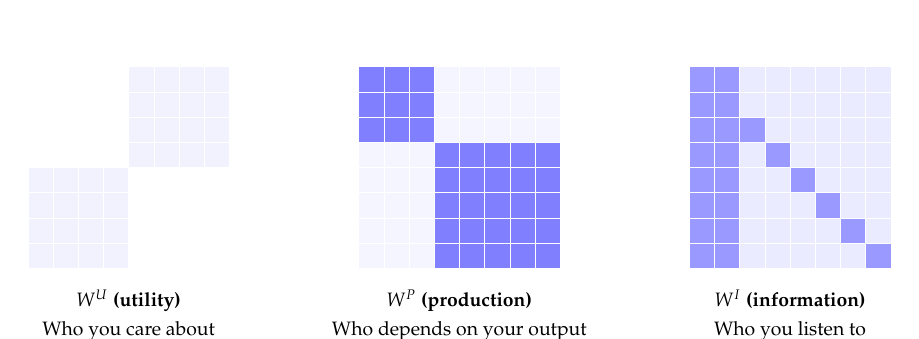
\begin{tikzpicture}[scale=1]
\def\N{8}
\def\s{0.32}

%% W^U: clustered (compadrazgo bonds within groups, weak across)
\foreach \i in {1,...,\N} {
  \foreach \j in {1,...,\N} {
    \pgfmathparse{
      (\i<=4 && \j<=4 && \i!=\j) ? 55 :
      (\i>4 && \j>4 && \i!=\j) ? 45 :
      (\i==\j) ? 0 :
      5
    }
    \edef\bp{\pgfmathresult}
    \fill[blue!\bp, draw=white, line width=0.1pt]
      ({(\j-1)*\s}, {(\N-\i)*\s}) rectangle +(\s,\s);
  }
}
\node[below, font=\scriptsize\bfseries] at ({4*\s}, -0.15) {$W^U$ (utility)};
\node[below, font=\scriptsize] at ({4*\s}, -0.55) {Who you care about};

%% W^P: block-diagonal (enclave)
\begin{scope}[xshift=4.2cm]
\foreach \i in {1,...,\N} {
  \foreach \j in {1,...,\N} {
    \pgfmathparse{
      (\i<=3 && \j<=3) ? 65 :
      (\i>3 && \j>3) ? 50 :
      4
    }
    \edef\bp{\pgfmathresult}
    \fill[blue!\bp, draw=white, line width=0.1pt]
      ({(\j-1)*\s}, {(\N-\i)*\s}) rectangle +(\s,\s);
  }
}
\node[below, font=\scriptsize\bfseries] at ({4*\s}, -0.15) {$W^P$ (production)};
\node[below, font=\scriptsize] at ({4*\s}, -0.55) {Who depends on your output};
\end{scope}

%% W^I: star-like (media concentrated)
\begin{scope}[xshift=8.4cm]
\foreach \i in {1,...,\N} {
  \foreach \j in {1,...,\N} {
    \pgfmathparse{
      (\j==1) ? 55 :
      (\j==2) ? 35 :
      (\i==\j) ? 40 :
      8
    }
    \edef\bp{\pgfmathresult}
    \fill[blue!\bp, draw=white, line width=0.1pt]
      ({(\j-1)*\s}, {(\N-\i)*\s}) rectangle +(\s,\s);
  }
}
\node[below, font=\scriptsize\bfseries] at ({4*\s}, -0.15) {$W^I$ (information)};
\node[below, font=\scriptsize] at ({4*\s}, -0.55) {Who you listen to};
\end{scope}
\end{tikzpicture}
\end{center}
\vspace{-0.5em}
\small Same eight agents, three different networks. $W^U$ is clustered (two social groups, caring mostly within). $W^P$ is block-diagonal (enclave: three agents in the modern sector, five in the traditional). $W^I$ is star-shaped (two media sources dominate everyone's attention). The three heatmaps have different topologies --- the agent who is central in one may be peripheral in another. The composite $W = \alpha_U W^U + \alpha_P W^P + \alpha_I W^I$ blends all three.
\end{vizpanel}


\subsection{When the Networks Align}

In the simplest case, all three networks are the same: $W^U = W^P = W^I = W$. Your friends are your business partners are your information sources. This is the world of a small village: the same 50 people appear in all three matrices.

When the networks align, the analysis simplifies dramatically: there is one weight matrix, one Perron eigenvector, one spectral gap. Power is power across all channels. The salte\~{n}a vendor who is central in the utility network is also central in the production network and the information network. Life is simple and oppressive.

\subsection{When the Networks Diverge}

In a complex economy, the three networks diverge. Your production network (the global supply chain) has nothing to do with your utility network (your family in Cochabamba) or your information network (TikTok, the Banco Central, your teacher).

This divergence creates both opportunities and tensions:

\textbf{Opportunity}: You can be peripheral in $W^P$ (a quinoa farmer in Oruro) but central in $W^I$ (a TikTok influencer with 200,000 followers). Information power can compensate for production powerlessness --- Luisa's phone gives her access to signals about the modern sector even though her production network is entirely traditional.

\textbf{Tension}: You can be central in $W^P$ (the YPFB gas engineer) but peripheral in $W^U$ (she moved to Tarija for work, leaving her family in Cochabamba). Economic success coexists with social isolation. The production network rewards one location; the utility network rewards another.

\textbf{Structural trap}: When $W^P$ is block-diagonal (Pinto) AND $W^I$ is block-diagonal (traditional-sector people attend only to traditional-sector signals), the two networks reinforce each other. Growth in the modern sector does not propagate through production ($W^P$ disconnected) AND does not propagate through information ($W^I$ disconnected). The trap is double-locked. Breaking it requires changing both matrices --- which is why structural policy is harder than it looks.


%% =====================================================================
\section{Canonical Topologies}
\label{sec:topologies}
%% =====================================================================

Any of the three networks can have any topology. But certain topologies appear again and again across economic settings. We catalog the most important ones and develop intuition for reading their structural properties.

(Readers should consult the interactive \textit{Seeing the Structure} companion tool, which visualizes all topologies below for $N = 3$ to $100$.)

\subsection{Complete (Anonymous Symmetric)}

$W = \frac{1}{N}\ones\ones'$. Every entry is $1/N$. Doubly stochastic, symmetric, rank 1, maximal spectral gap $\Gamma = 1$, equal Perron eigenvector $\boldsymbol{\pi} = \frac{1}{N}\ones$.

\textit{As $W^U$:} universal, symmetric altruism. You care about everyone equally.

\textit{As $W^P$:} every sector uses every other sector's output in equal proportion. No specialization, no comparative advantage, no structural heterogeneity. Unrealistic but useful as a benchmark.

\textit{As $W^I$:} you listen to everyone equally. No opinion leaders, no media concentration, no filter bubbles. Information aggregates to the simple average of initial beliefs.

\textit{Economics:} The welfare theorems hold. The First Welfare Theorem says: if $W^U = 0$ and $W^P = \frac{1}{N}\ones\ones'$, the competitive equilibrium is Pareto efficient. This is the standard result. It is the structural content of ``perfect competition.''


\subsection{Star (Hub-Spoke)}

One hub ($h$) connected to all spokes; spokes connected only to the hub.
\begin{equation}
W_{ih} \text{ large for all } i \neq h; \qquad W_{ij} \approx 0 \text{ for } i, j \neq h.
\end{equation}

Spectral gap $\Gamma \approx 0$. Perron eigenvector concentrates on the hub: $\pi_h \gg \pi_i$ for $i \neq h$.

\textit{As $W^U$:} everyone cares about the hub (celebrity, patron, chief), nobody cares about each other. Patron-client structures, populist politics.

\textit{As $W^P$:} all production passes through a single firm or sector (the platform, the middleman, the colonial trading company). Amazon, the East India Company.

\textit{As $W^I$:} one source broadcasts, all others listen. State media, monopoly news, papal authority. The long-run consensus equals the hub's initial belief. Epistemic dictatorship.


\subsection{Block-Diagonal (Dual Economy)}

Two or more blocks with strong internal links and weak cross-block links.
\begin{equation}
W \approx \begin{pmatrix} W_{11} & \varepsilon \\ \varepsilon' & W_{22} \end{pmatrix}, \quad \|\varepsilon\| \ll \|W_{11}\|, \|W_{22}\|.
\end{equation}

Small spectral gap $\Gamma \approx |\rho(W_{11}) - \rho(W_{22})|$. Perron eigenvector concentrates on the block with higher spectral radius.

\textit{As $W^U$:} two social groups that care about their own members but not about the other group. Ethnic enclaves, caste, class segregation.

\textit{As $W^P$:} Pinto's structural heterogeneity. The modern sector and the traditional sector, barely connected. Bolivia's gas and quinoa economies. Growth does not propagate (Chapter~3).

\textit{As $W^I$:} two information ecosystems. Rural and urban. Spanish-language and Quechua-language. Fox News and MSNBC. Each group converges to its own consensus internally, but the two groups' consensuses may diverge. This is the formation-level mechanism of structural reproduction: if traditional-sector people attend only to traditional-sector signals, their beliefs about returns are calibrated to the traditional sector, which reproduces traditional-sector behavior, which keeps them in the traditional sector.


\subsection{Core-Periphery (Prebisch)}

A dense core and a sparse periphery, with asymmetric links: periphery depends on core, core barely depends on periphery.
\begin{equation}
W_{ij} \text{ large for } i \in \text{periphery}, j \in \text{core}; \qquad W_{ij} \approx 0 \text{ for } i \in \text{core}, j \in \text{periphery}.
\end{equation}

Perron eigenvector assigns high weight to the core and low weight to the periphery: $\pi_{\text{core}} \gg \pi_{\text{periphery}}$.

\textit{As $W^U$:} the periphery admires and envies the center; the center is indifferent to the periphery. Colonial relations, celebrity culture, academic prestige hierarchies.

\textit{As $W^P$:} Prebisch's center-periphery. The periphery exports raw materials to the center and imports manufactures. The Leontief multiplier is high for the center (column sums of $(I - \gamma W^P)^{-1}$ are large) and low for the periphery. Terms of trade deterioration is a spectral property of this asymmetric $W^P$ (Chapter~16).

\textit{As $W^I$:} the periphery absorbs signals from the center (economic theory, cultural norms, consumption patterns, policy advice) but not vice versa. The long-run consensus converges to center beliefs. The Washington Consensus as a DeGroot equilibrium.


\subsection{Other Topologies}

Several additional topologies appear in applications:

\textbf{Ring} (supply chain): Each agent connects to neighbors. Sequential production. Shocks propagate slowly along the chain. Manufacturing assembly lines, agricultural value chains.

\textbf{Hierarchy} (tree): Top-down connections. Firms, bureaucracies, military, caste. Power decreases monotonically with depth in the tree. Information flows down; surplus flows up.

\textbf{Small-world}: Local clusters plus random long-range shortcuts. Most social networks exhibit this structure (Watts and Strogatz, 1998). High clustering with short path lengths. Ideas diffuse faster than in a ring but less uniformly than in a complete graph.

\textbf{Scale-free}: Few super-connected hubs, many weakly connected nodes. Power-law degree distribution. Wealth, internet, citation networks. Extreme power concentration in the Perron eigenvector.

\textbf{Random} (Erd\H{o}s-R\'{e}nyi): Each link exists with probability $p$. No structure by design. Useful as a null model: any deviation from random IS structure.


%% =====================================================================
\section{The Composite Weight Matrix}
\label{sec:composite}
%% =====================================================================

In many applications, the three networks operate simultaneously and interact. We define the composite.

\begin{definition}[Composite Weight Matrix]\label{def:composite}
The \textbf{composite weight matrix} is:
\begin{equation}\label{eq:composite}
W = \alpha_U W^U + \alpha_P W^P + \alpha_I W^I, \quad \alpha_U + \alpha_P + \alpha_I = 1,
\end{equation}
where $\alpha_U, \alpha_P, \alpha_I \geq 0$ are the relative importance of each channel.
\end{definition}

The composite $W$ is the single matrix that summarizes the overall structure of economic interaction. Its Perron eigenvector $\boldsymbol{\pi}(W)$ is the \textbf{power vector}: agent $i$'s structural power is $\pi_i$, determined jointly by her position in all three networks.

\begin{proposition}[Power from the Composite]\label{prop:composite_power}
If $W$ is irreducible and aperiodic, the left Perron eigenvector $\boldsymbol{\pi}$ of the composite $W$ satisfies:
\begin{equation}
\pi_i = \alpha_U \sum_j \pi_j W^U_{ji} + \alpha_P \sum_j \pi_j W^P_{ji} + \alpha_I \sum_j \pi_j W^I_{ji}.
\end{equation}
An agent's power is the weighted sum of power directed toward her through all three channels: how much powerful agents care about her (utility channel), how much powerful agents depend on her output (production channel), and how much powerful agents listen to her signals (information channel).
\end{proposition}

\begin{intuition}[What determines power]
Your structural power $\pi_i$ is high if:
\begin{enumerate}
\item People who care about you ($W^U_{ji}$ large) are themselves powerful.
\item People who depend on your output ($W^P_{ji}$ large) are themselves powerful.
\item People who listen to your signals ($W^I_{ji}$ large) are themselves powerful.
\end{enumerate}
This is recursive: power begets power, through the Perron eigenvector's self-referential definition. This is the mathematical content of ``privilege reproduces itself.'' It is not a moral judgment. It is a theorem about nonnegative matrices.
\end{intuition}

\begin{example}[Power in La Paz]\label{ex:LaPaz}
Consider three agents: a Cabinet Minister ($i=1$), a Gas Executive ($i=2$), and a Market Vendor ($i=3$).

Utility network (who cares about whom):
\begin{equation}
W^U = \begin{pmatrix} 0 & 0.3 & 0.0 \\ 0.2 & 0 & 0.0 \\ 0.0 & 0.0 & 0 \end{pmatrix}.
\end{equation}
The Minister and the Executive care about each other. Nobody cares about the Vendor.

Production network (who depends on whose output):
\begin{equation}
W^P = \begin{pmatrix} 0.1 & 0.4 & 0.1 \\ 0.3 & 0.2 & 0.0 \\ 0.0 & 0.0 & 0.3 \end{pmatrix}.
\end{equation}
The Minister depends on gas revenue (0.4 weight on Executive). The Executive depends on regulatory approval (0.3 weight on Minister). The Vendor is self-contained.

Information network (who listens to whom):
\begin{equation}
W^I = \begin{pmatrix} 0.3 & 0.5 & 0.2 \\ 0.4 & 0.3 & 0.3 \\ 0.2 & 0.1 & 0.7 \end{pmatrix}.
\end{equation}
The Minister listens mostly to the Executive. The Executive listens to the Minister and somewhat to the Vendor (market prices as signal). The Vendor listens mostly to herself (local knowledge).

Composite ($\alpha_U = 0.2, \alpha_P = 0.5, \alpha_I = 0.3$):
\begin{equation}
W = 0.2 W^U + 0.5 W^P + 0.3 W^I = \begin{pmatrix} 0.14 & 0.41 & 0.11 \\ 0.27 & 0.19 & 0.09 \\ 0.06 & 0.03 & 0.36 \end{pmatrix}.
\end{equation}

The left Perron eigenvector (computed numerically): $\boldsymbol{\pi} \approx (0.40, 0.38, 0.22)$. The Minister has the most power (0.40), followed closely by the Executive (0.38). The Vendor has some power (0.22) --- mostly from her information self-reliance --- but substantially less than either.

This is the power structure of La Paz in three numbers.
\end{example}

\begin{vizpanel}{La Paz: three networks and their composite}
\begin{center}
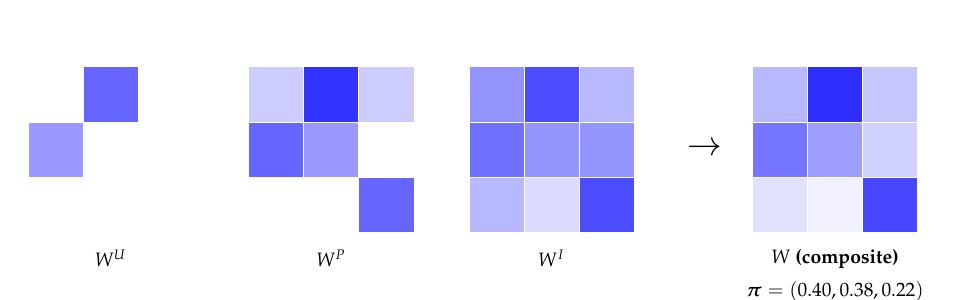
\begin{tikzpicture}[scale=1]
\def\s{0.7}
%% W^U
\foreach \i/\j/\v in {1/1/0,1/2/60,1/3/0,2/1/40,2/2/0,2/3/0,3/1/0,3/2/0,3/3/0} {
  \fill[blue!\v, draw=white, line width=0.2pt]
    ({(\j-1)*\s}, {(3-\i)*\s}) rectangle +(\s,\s);
}
\node[below, font=\scriptsize\bfseries] at ({1.5*\s}, -0.1) {$W^U$};

%% W^P
\begin{scope}[xshift=2.8cm]
\foreach \i/\j/\v in {1/1/20,1/2/80,1/3/20,2/1/60,2/2/40,2/3/0,3/1/0,3/2/0,3/3/60} {
  \fill[blue!\v, draw=white, line width=0.2pt]
    ({(\j-1)*\s}, {(3-\i)*\s}) rectangle +(\s,\s);
}
\node[below, font=\scriptsize\bfseries] at ({1.5*\s}, -0.1) {$W^P$};
\end{scope}

%% W^I
\begin{scope}[xshift=5.6cm]
\foreach \i/\j/\v in {1/1/60,1/2/100,1/3/40,2/1/80,2/2/60,2/3/60,3/1/40,3/2/20,3/3/100} {
  \pgfmathparse{\v*0.7}
  \edef\bp{\pgfmathresult}
  \fill[blue!\bp, draw=white, line width=0.2pt]
    ({(\j-1)*\s}, {(3-\i)*\s}) rectangle +(\s,\s);
}
\node[below, font=\scriptsize\bfseries] at ({1.5*\s}, -0.1) {$W^I$};
\end{scope}

%% Arrow
\node[font=\large] at (8.6, 1.05) {$\to$};

%% Composite W
\begin{scope}[xshift=9.2cm]
\foreach \i/\j/\v in {1/1/28,1/2/82,1/3/22,2/1/54,2/2/38,2/3/18,3/1/12,3/2/6,3/3/72} {
  \fill[blue!\v, draw=white, line width=0.2pt]
    ({(\j-1)*\s}, {(3-\i)*\s}) rectangle +(\s,\s);
}
\node[below, font=\scriptsize\bfseries] at ({1.5*\s}, -0.1) {$W$ (composite)};
\node[below, font=\scriptsize] at ({1.5*\s}, -0.5) {$\boldsymbol{\pi} = (0.40, 0.38, 0.22)$};
\end{scope}
\end{tikzpicture}
\end{center}
\vspace{-0.5em}
\small The La Paz economy: Minister, Gas Executive, Market Vendor. Three component networks with different topologies blend into the composite. Column 2 of $W^P$ is brightest (everyone depends on the Executive's output). Column 3 of $W^I$ is dimmer (nobody much listens to the Vendor). The composite $\boldsymbol{\pi}$: Minister 40\%, Executive 38\%, Vendor 22\%. The Vendor's self-reliance in $W^I$ saves her from zero power, but she is structurally marginal.
\end{vizpanel}


%% =====================================================================
\section{What the Standard Model Assumes}
\label{sec:standard_revisited}
%% =====================================================================

We can now state precisely what the standard competitive model assumes about the three networks.

\begin{proposition}[The Standard Model as a Network Assumption]\label{prop:standard}
The standard competitive model assumes:
\begin{enumerate}
\item $W^U = 0$ (no utility externalities).
\item $W^P$ is given by technology (the input-output matrix, taken as data).
\item $W^I$ does not exist (preferences and beliefs are exogenous and common knowledge).
\item The market interaction is $W^{\text{market}} = \frac{1}{N}\ones\ones'$ (prices aggregate demands anonymously and symmetrically).
\end{enumerate}
Under these assumptions, the welfare theorems hold, the competitive equilibrium is Pareto efficient, and social structure is irrelevant.

Structural economics relaxes each assumption:
\begin{enumerate}
\item General $W^U$ (utility externalities matter for welfare, efficiency, and policy).
\item General $W^P$ (the topology of production determines growth propagation and structural change).
\item General $W^I$ (information flows shape beliefs and preferences, reproducing or disrupting the structure).
\item The market interaction is mediated by all three networks, not just by anonymous prices.
\end{enumerate}
\end{proposition}

This is the complete structural program. The rest of the book develops each relaxation: Chapter~6 derives power from $W$, Chapter~7 derives the bargaining equilibrium, Chapter~8 develops belief manipulation through $W^I$, and Chapters~9--12 develop the formation model where $W^I$ shapes preferences.


%% =====================================================================
\section{Summary}
\label{sec:summary}
%% =====================================================================

\begin{enumerate}
\item The economy is organized by three networks: $W^U$ (utility externalities), $W^P$ (production spillovers), and $W^I$ (information flows). The standard model ignores the first, measures the second, and denies the existence of the third.

\item $W^U$ captures who affects your happiness. It enters utility directly: $V_i = U_i + \gamma_U \sum_j W^U_{ij} U_j$. The standard model assumes $W^U = 0$, which means nobody's consumption affects anyone else.

\item $W^P$ captures who depends on whose output. It determines the Leontief inverse $(I - \gamma_P W^P)^{-1}$, which amplifies shocks through inter-sectoral linkages. This is the matrix from Chapters~1 and 3, now recognized as one of three structural objects.

\item $W^I$ captures who listens to whom. It drives belief dynamics through DeGroot learning: $\mathbf{b}^{(t+1)} = W^I \mathbf{b}^{(t)}$, converging to a consensus weighted by the Perron eigenvector $\boldsymbol{\pi}(W^I)$. This is epistemic power.

\item The composite $W = \alpha_U W^U + \alpha_P W^P + \alpha_I W^I$ summarizes the full structure. Its Perron eigenvector is the power vector. Power is recursive: it comes from being valued, depended upon, and listened to by other powerful agents.

\item Canonical topologies --- complete, star, block-diagonal, core-periphery, ring, hierarchy, small-world, scale-free, random --- characterize the qualitative features of each network. The topology determines the spectral properties, which determine propagation, convergence, power concentration, and structural persistence.
\end{enumerate}


%% =====================================================================
\section{Exercises}
\label{sec:exercises}
%% =====================================================================

\begin{enumerate}[label=\textbf{5.\arabic*}, leftmargin=3em]

\item \textbf{Utility externalities.} For the three-vendor economy (Example~\ref{ex:vendors}), with $\gamma_U = 0.5$:
\begin{enumerate}
\item Compute $V_2$ and $V_3$ (Rosa's and Carlos's social utilities).
\item A social planner maximizes $\sum_i V_i$. Show that the planner's optimal allocation differs from the competitive equilibrium (which maximizes $\sum_i U_i$). Who gets more under the planner?
\item What happens as $\gamma_U \to 1$? As $\gamma_U \to 0$?
\end{enumerate}

\item \textbf{Three networks for a factory town.} A town has $N = 4$ agents: Factory Owner ($F$), Worker ($W$), Shopkeeper ($S$), Mayor ($M$).
\begin{enumerate}
\item Write plausible $W^U$, $W^P$, and $W^I$ matrices (each $4 \times 4$).
\item Compute the composite $W$ with equal weights $\alpha = 1/3$.
\item Find the Perron eigenvector. Who has the most power? Explain why.
\item Now suppose the factory closes. Which entries of $W^P$ go to zero? How does the Perron eigenvector change?
\end{enumerate}

\item \textbf{DeGroot learning.} For $N = 3$ with:
\begin{equation}
W^I = \begin{pmatrix} 0.5 & 0.3 & 0.2 \\ 0.1 & 0.6 & 0.3 \\ 0.2 & 0.2 & 0.6 \end{pmatrix}.
\end{equation}
\begin{enumerate}
\item Verify $W^I$ is row-stochastic.
\item Compute $(W^I)^2$ and $(W^I)^5$ (use Python). Are the rows becoming more similar?
\item Find the left Perron eigenvector $\boldsymbol{\pi}$. Which agent has the most epistemic power?
\item Starting from $\mathbf{b}^{(0)} = (0, 0.5, 1)'$, compute $\mathbf{b}^{(t)}$ for $t = 1, 2, 5, 10, 50$. Verify convergence to $\boldsymbol{\pi}'\mathbf{b}^{(0)}$.
\end{enumerate}

\item \textbf{The phone as structural change.} Luisa's pre-phone $W^I$ and post-phone $W^I$ from Example~\ref{ex:Luisa}. Extend to $N = 5$ agents (Mother, Friend, Cousin, TikTok, Teacher) where each agent also has a $W^I$ row (Mother listens to: herself 0.6, friend 0.2, teacher 0.2; etc.).
\begin{enumerate}
\item Construct the full $5 \times 5$ pre-phone and post-phone $W^I$.
\item Compute the Perron eigenvector for both. How does epistemic power shift?
\item If initial beliefs about ``returns to education'' are $\mathbf{b}^{(0)} = (0.3, 0.3, 0.8, 0.6, 0.7)$ (Mother and Friend think returns are low; Cousin, TikTok, Teacher think returns are high), what is the long-run consensus pre-phone? Post-phone?
\item Interpret: how much does the phone change Luisa's long-run belief about education?
\end{enumerate}

\item \textbf{When networks align.} Construct a $4 \times 4$ economy where $W^U = W^P = W^I$ (a village where everyone is simultaneously your friend, your supplier, and your information source).
\begin{enumerate}
\item Compute the composite $W$. Note: it equals each component matrix.
\item Now perturb: add one external production link (agent 1 begins importing from outside). How does $W^P$ change? How does the composite change? What happens to the Perron eigenvector?
\item Interpret: what does it mean for a village to enter the global supply chain?
\end{enumerate}

\item \textbf{Prebisch in $W^I$.} Construct a $6 \times 6$ global $W^I$: agents 1--2 are ``center'' countries, agents 3--6 are ``periphery'' countries. Center listens mostly to itself; periphery listens mostly to center.
\begin{enumerate}
\item Compute the Perron eigenvector. How much epistemic power do center countries have?
\item Initial beliefs about ``the optimal tariff policy'': center believes $b = 0$ (free trade), periphery believes $b = 1$ (protection). What is the long-run consensus?
\item What fraction of the consensus is determined by the center? Is this consistent with the Washington Consensus?
\item What would it take (in terms of $W^I$ entries) for the periphery's belief to survive?
\end{enumerate}

\item \textbf{Bolivia: composite power.} Using Bolivia's three-agent model (Example~\ref{ex:LaPaz}):
\begin{enumerate}
\item Vary $\alpha_P$ from 0 to 1 (holding $\alpha_U / \alpha_I$ constant). Plot $\pi_3$ (Vendor's power) as a function of $\alpha_P$. When does the Vendor have the most power? The least?
\item Interpret: in what kind of economy does the market vendor matter most? When does she become invisible?
\item Add a fourth agent: ``Luisa (Student).'' Construct plausible $W^U$, $W^P$, $W^I$ rows for Luisa. How does her inclusion change the power structure?
\end{enumerate}

\end{enumerate}


%% =====================================================================
\newpage
\section*{Mathematical Appendices}
\addcontentsline{toc}{section}{Mathematical Appendices}
%% =====================================================================

\subsection*{Appendix 5A: Graph Theory for Economists}
\addcontentsline{toc}{subsection}{Appendix 5A: Graph Theory for Economists}
\label{app:graphs}

A \textbf{directed graph} (digraph) $G = (V, E)$ consists of a set of \textit{vertices} (nodes, agents) $V = \{1, \ldots, N\}$ and a set of \textit{edges} (links, connections) $E \subseteq V \times V$. An edge $(i, j)$ means agent $i$ is connected to agent $j$.

Every $N \times N$ weight matrix $W$ defines a weighted directed graph: the vertices are agents $1, \ldots, N$, and the edge from $j$ to $i$ has weight $W_{ij}$. (Convention: $W_{ij} > 0$ means there is an edge from $j$ to $i$, i.e., $j$ affects $i$.)

\paragraph{Key definitions.}

\textit{Path}: a sequence of edges connecting $i$ to $j$. The \textit{length} of a path is the number of edges. A path of length $k$ from $j$ to $i$ exists if and only if $(W^k)_{ij} > 0$: the $(i,j)$ entry of the $k$-th power of $W$.

\textit{Connected}: $i$ can reach $j$ through a path of some finite length. \textit{Strongly connected}: every agent can reach every other agent. Equivalently, $W$ is \textit{irreducible}: $(I + W)^{N-1}$ has all positive entries.

\textit{Aperiodic}: the greatest common divisor of the lengths of all cycles through any agent is 1. Sufficient condition: some diagonal entry $W_{ii} > 0$ (some agent has a self-loop, i.e., some of their influence stays with themselves).

\textit{Why these matter}: The Perron-Frobenius theorem (Chapter~6) requires $W$ to be nonnegative. Strong connectivity ensures a unique Perron eigenvector. Aperiodicity ensures convergence of $(W^t)$ to a limit (the consensus matrix $\ones\boldsymbol{\pi}'$). Without strong connectivity, the network fragments into components, each with its own Perron eigenvector. Without aperiodicity, the system cycles rather than converging.

\paragraph{Degree and centrality.}

\textit{In-degree}: $d_i^{\text{in}} = \sum_j W_{ij}$ (row sum). How much total influence agent $i$ receives. For row-stochastic $W^I$: always 1.

\textit{Out-degree}: $d_i^{\text{out}} = \sum_j W_{ji}$ (column sum). How much total influence agent $i$ exerts. Not necessarily 1 even for row-stochastic matrices.

\textit{Eigenvector centrality}: the Perron eigenvector $\boldsymbol{\pi}$ assigns each agent a centrality proportional to the centrality of agents who point toward her. This is the recursive ``power'' we have been developing. It is not the same as degree (a node can have high degree but low eigenvector centrality if its neighbors are peripheral). Chapter~6 develops this fully.

\paragraph{Adjacency matrix vs.\ weight matrix.}

The \textit{adjacency matrix} $A$ is binary: $A_{ij} = 1$ if there is an edge from $j$ to $i$, and $0$ otherwise. The \textit{weight matrix} $W$ generalizes this: $W_{ij} \geq 0$ is the strength of the edge. In this book, we always use weight matrices. The adjacency matrix is the special case where all edges have weight 1.


\subsection*{Appendix 5B: Stochastic Matrices and the Perron Eigenvector}
\addcontentsline{toc}{subsection}{Appendix 5B: Stochastic Matrices and the Perron Eigenvector}
\label{app:stochastic}

\paragraph{Row-stochastic matrices.} A nonnegative matrix $W$ is \textbf{row-stochastic} if $W\ones = \ones$: every row sums to 1. This means each row is a probability distribution. In the context of $W^I$, row-stochasticity means each agent allocates 100\% of her attention across all agents (including possibly herself).

\paragraph{Key property.} If $W$ is row-stochastic, then $\rho(W) = 1$ and $\ones$ is a right eigenvector: $W\ones = 1 \cdot \ones$.

\paragraph{The left Perron eigenvector.} The left eigenvector corresponding to eigenvalue 1 is $\boldsymbol{\pi}$: the vector satisfying $\boldsymbol{\pi}'W = \boldsymbol{\pi}'$ with $\boldsymbol{\pi} \geq 0$ and $\ones'\boldsymbol{\pi} = 1$. For a row-stochastic matrix, $\boldsymbol{\pi}$ is also the \textit{stationary distribution} of the Markov chain defined by $W$: if you start at a random node drawn from $\boldsymbol{\pi}$ and take a random step according to $W$, you remain distributed according to $\boldsymbol{\pi}$.

\paragraph{Why left, not right?} The right eigenvector of a row-stochastic matrix is always $\ones$ --- uninformative. The left eigenvector is the interesting object: it tells you which agents have the most influence in the long run. ``Left Perron'' is the power vector throughout this book.

\paragraph{Computing $\boldsymbol{\pi}$ by iteration.} Start with any positive vector $\mathbf{v}^{(0)}$. Iterate: $\mathbf{v}^{(t+1)\prime} = \mathbf{v}^{(t)\prime} W$. Normalize: $\boldsymbol{\pi}^{(t)} = \mathbf{v}^{(t)} / \|\mathbf{v}^{(t)}\|_1$. If $W$ is irreducible and aperiodic, $\boldsymbol{\pi}^{(t)} \to \boldsymbol{\pi}$ as $t \to \infty$. Convergence is geometric at rate $|\lambda_2(W)|$, the second-largest eigenvalue in magnitude. Faster convergence means larger spectral gap $\Gamma = 1 - |\lambda_2|$.

\paragraph{Example.} For the $3 \times 3$ matrix from Exercise~5.3:
\begin{equation}
W^I = \begin{pmatrix} 0.5 & 0.3 & 0.2 \\ 0.1 & 0.6 & 0.3 \\ 0.2 & 0.2 & 0.6 \end{pmatrix}.
\end{equation}

Starting from $\mathbf{v}^{(0)} = (1, 1, 1)$:
\begin{center}
\begin{tabular}{lcccc}
\toprule
$t$ & $\pi_1$ & $\pi_2$ & $\pi_3$ & Max change \\
\midrule
0 & 0.333 & 0.333 & 0.333 & --- \\
1 & 0.267 & 0.367 & 0.367 & 0.067 \\
2 & 0.244 & 0.374 & 0.382 & 0.023 \\
5 & 0.232 & 0.375 & 0.394 & 0.002 \\
$\infty$ & 0.231 & 0.375 & 0.395 & 0 \\
\bottomrule
\end{tabular}
\end{center}

Agent 3 has the most epistemic power (0.395), despite not having the highest self-weight (that's agent 2 with $W^I_{22} = 0.6$). Why? Because agents 1 and 2 both listen to agent 3 more than agent 3 listens to them. Structural position, not self-confidence, determines power.

\paragraph{Doubly stochastic matrices.} If $W$ is both row-stochastic AND column-stochastic ($\ones'W = \ones'$), then $\boldsymbol{\pi} = \frac{1}{N}\ones$: all agents have equal power. This is the competitive benchmark from Chapter~1 ($W^{CE} = \frac{1}{N}\ones\ones'$ is doubly stochastic). Any deviation from doubly stochastic generates power asymmetry.


%% =====================================================================

\subsection*{Structuralist Case Study: Dos Santos's Three Regimes of the Weight Matrix}
\addcontentsline{toc}{subsection}{Structuralist Case Study: Dos Santos (1970)}

In 1970, Theot\^{o}nio dos Santos published ``The Structure of Dependence'' in the \textit{American Economic Review} --- a six-page paper presented at an AEA panel on ``Economics of Imperialism'' chaired by Paul Sweezy. The paper's core contribution was a \textbf{taxonomy of three historical forms of dependence}, each corresponding to a specific phase of world capitalist development. Read through this chapter's framework, the three forms are three historical regimes of the weight matrix $W$.

\textbf{Regime 1: Colonial dependence (trade-export).} The metropole extracts raw materials from the colony through monopoly control of land, mines, and labor. The weight matrix is a \textbf{star graph}: all edges point to the colonial power. $W^P$ has one bright column (the metropole) and $N-1$ dim columns (the colonies). The colonies do not trade with each other --- the off-diagonal entries among periphery nodes are zero. $W^I$ is similarly star-shaped: information (prices, technology, legal frameworks) flows from the metropole to the colonies, not between colonies. Power is maximally concentrated: $\boldsymbol{\pi} \approx (1, 0, \ldots, 0)$.

\textbf{Regime 2: Financial-industrial dependence (late 19th century).} Big capital invests in raw material and agricultural production for export to hegemonic centers. The star becomes a \textbf{hub-spoke with multiple hubs}: several industrial powers (Britain, France, the US) each have their own peripheral suppliers. $W^P$ now has a few bright columns instead of one. The periphery begins to develop limited internal linkages (railways for commodity transport, ports, basic processing), adding small off-diagonal entries among peripheral nodes. But the dominant flows still point toward the center. $W^I$ remains center-dominated: economic policy knowledge flows from London and New York.

\textbf{Regime 3: Technological-industrial dependence (post-WWII).} Multinational corporations invest in industries oriented toward the internal market of the underdeveloped countries. The topology becomes more complex: MNCs create \textbf{bridging nodes} that connect the domestic $W^P$ to the global $W^P$ through intra-firm trade. The domestic matrix acquires new blocks (the MNC-owned modern sector), but these blocks connect outward to headquarters rather than inward to the traditional domestic sector. This is Sunkel's ``transnational integration and national disintegration'' as a matrix rewiring: cross-country edges among elite nodes strengthen while within-country edges between modern and traditional blocks weaken. The information network $W^I$ becomes layered: the MNC subsidiary receives technical knowledge from headquarters ($W^I_{\text{subsidiary, HQ}}$ large) but does not transmit local knowledge back ($W^I_{\text{HQ, subsidiary}} \approx 0$).

\begin{center}
\begin{tabular}{llll}
\toprule
\textbf{Dos Santos's regime} & \textbf{Topology of $W$} & \textbf{Power structure} & \textbf{$\Gamma$} \\
\midrule
Colonial & Star & $\pi_{\text{metropole}} \approx 1$ & $\approx 0$ \\
Financial-industrial & Multi-hub & $\pi_{\text{centers}} \gg \pi_{\text{periphery}}$ & Small \\
Technological-industrial & Complex asymmetric & $\pi_{\text{MNC}} > \pi_{\text{domestic elite}} \gg \pi_{\text{traditional}}$ & Small \\
\bottomrule
\end{tabular}
\end{center}

The taxonomy's power is its specificity: each regime generates a \textit{different} heatmap, a different Perron eigenvector, and a different spectral gap, even though all three are ``dependent.'' The colonial heatmap has one blazing column. The financial-industrial heatmap has several bright columns and dim periphery. The technological-industrial heatmap has a complex block structure with MNC bridging nodes creating cross-border links while domestic cross-block links remain dark.

Dos Santos's definition --- ``a situation in which the economy of certain countries is conditioned by the development and expansion of another economy'' --- is the statement that the Perron eigenvector of the global $W$ assigns dominant weight to the conditioning economy. The taxonomy refines this: \textit{how} the conditioning occurs (through which channel of $W$ and with which topology) determines the specific developmental consequences. The colonial star produces extraction. The financial hub-spoke produces commodity dependence. The technological-industrial complex produces what Pinto called ``modernizaci\'{o}n excluyente'' --- a modern sector that connects to the world but not to its own country.

The three networks of this chapter --- $W^U$, $W^P$, $W^I$ --- are the analytical tools that Dos Santos needed but did not have. His taxonomy describes what the matrices look like. The Perron eigenvector tells you who benefits.


\subsection*{Further Reading}
\addcontentsline{toc}{subsection}{Further Reading}

\textbf{Social preferences and externalities:} Fehr and Schmidt (1999), ``A Theory of Fairness, Competition, and Cooperation,'' \textit{QJE}. Sobel (2005), ``Interdependent Preferences and Reciprocity,'' \textit{JEL}. Bowles and Gintis (2011), \textit{A Cooperative Species}.

\textbf{Production networks:} See readings from Chapters~1 and~3. The comprehensive reference is now Carvalho and Tahbaz-Salehi (2019), ``Production Networks: A Primer,'' \textit{Annual Review of Economics}.

\textbf{DeGroot learning:} DeGroot (1974), ``Reaching a Consensus.'' Golub and Jackson (2010), ``Na\"{i}ve Learning in Social Networks and the Wisdom of Crowds,'' \textit{AEJ: Microeconomics}. This is the key paper on convergence, influence, and the Perron eigenvector in learning models.

\textbf{Network economics textbooks:} Jackson (2008), \textit{Social and Economic Networks}. Goyal (2023), \textit{Networks: An Economics Approach}. Sargent and Stachurski (2024), \textit{Economic Networks}.

\textbf{The interaction of multiple networks:} Kivel\"{a} et al.\ (2014), ``Multilayer Networks,'' \textit{Journal of Complex Networks}. For the economic application: the composite $W$ is related to the ``multiplex'' framework in network science.

\textbf{Prebisch and information dependency:} Prebisch (1950) on ideological dependency. Cardoso and Faletto (1969), \textit{Dependency and Development in Latin America}. For the modern formalization: Acemoglu et al.\ (2010), ``Spread of (Mis)information in Social Networks,'' \textit{Games and Economic Behavior}.

\textbf{Dependency theory:} Dos Santos (1970), ``The Structure of Dependence,'' \textit{AER} 60(2), pp.~231--236 (the six pages that define the taxonomy formalized in the case study above). Dos Santos (1978), \textit{Imperialismo y Dependencia}, M\'{e}xico: Era. Sunkel (1971), ``Capitalismo transnacional y desintegraci\'{o}n nacional,'' \textit{Estudios Internacionales} 4(16).


\end{document}
